\documentclass[12pt]{article}
\setlength{\oddsidemargin}{0in}
\setlength{\evensidemargin}{0in}
\setlength{\textwidth}{6.5in}
\setlength{\parindent}{0in}
\setlength{\parskip}{\baselineskip}

\usepackage{amsmath,amsfonts,amssymb,bm,graphics,pgfplots,framed,dsfont}
\usepackage[scale=0.75,top=1cm,bottom=3cm]{geometry}

\begin{document}

\textbf{Minh Anh Nguyen }\\
\textbf{Calculus 1 Assignment-6}\\
\textbf{Section: 04}\\
\textbf{TA's name: Arthur Huey}

\hrulefill

Section 3.1:

\begin{enumerate}
    \setcounter{enumi}{34}
    \item Find the critical numbers of the function.\\
        \[g(y) = \frac{y-1}{y^2-y+1}\]
        \[g'(y) = \frac{(y-1)'(y^2-y+1) - (y^2-y+1)'(y-1)}{(y^2-y+1)^2}\]
        \[g'(y) = \frac{y^2-y+1 - (2y-1)(y-1)}{(y^2-y+1)^2}\]
        \[g'(y) = \frac{y^2-y+1 - 2y^2+2y+y-1}{(y^2-y+1)^2}\]
        \[g'(y) = \frac{-y^2+2y}{(y^2-y+1)^2}\]
        \[-y^2+2y=0\]
        \[-y(y-2)=0\]
        \[y = 0 \text{ or } y = 2\]
        The critical numbers of the function are 0 and 2.
    \setcounter{enumi}{40}
    \item Find the critical numbers of the function.
        \[F(x) = x^{4/5}(x-2)^2\]
        \[F(x) = x^{4/5}(x^2-4x+4)\]
        \[F(x) = x^{14/5}-4x^{9/5}+4x^{4/5}\]
        \[F'(x) = \frac{14}{5}x^{9/5}-\frac{36}{5}x^{4/5}+\frac{16}{5}x^{-1/5}\]
        \[\frac{14}{5}x^{9/5}-\frac{36}{5}x^{4/5}+\frac{16}{5}x^{-1/5}=0\]
        \[x = \frac{4}{7} \text{ or } x = 2\]
        The critical numbers of the function are ${\displaystyle \frac{4}{7}}$ and 2.
    \newpage
    \setcounter{enumi}{44}
    \item Find the critical numbers of the function.
        \[f(\theta) = 2\cos\theta + \sin^2\theta\]
        \[f'(\theta) = -2\sin\theta + 2\sin\theta\cos\theta\]
        \[0 = -2\sin\theta + 2\sin\theta\cos\theta\]
        \[2\sin\theta = 2\sin\theta\cos\theta\]
        \[\theta = n\pi \text{ with n is a integer.}\]
        The critical numbers of the function are $n\pi$ with n is a integer.
    \setcounter{enumi}{52}
    \item Find the absolute maximum and absolute minimum values of $f$ on the given interval.
        \[f(x)=3x^4-4x^3-12x^2+1\text{, [-2,3]}\]
        \[f'(x)=12x^3-12x^2-24x\]
        \[12x^3-12x^2-24x=0\]
        \[12x(x^2-x-2)=0\]
        \[12x(x-2)(x+1)=0\]
        \[x = 0 \text{ or } x = 2 \text{ or } x=-1\]
        \[f(-2) = 33\]
        \[f(-1) = -4\]
        \[f(0) = 1\]
        \[f(2) = -31\]
        \[f(3) = 28\]
        The absolute maximum value of $f$ is 33 and the absolute minimum value of $f$ is -31.
    \setcounter{enumi}{58}
    \item Find the absolute maximum and absolute minimum values of $f$ on the given interval.
        \[f(t) = 2\cos t + \sin 2t, [0,\frac{\pi}{2}]\]
        \[f'(t) = -2\sin t + 2\cos 2t\]
        \[0 = -2\sin t + 2\cos 2t\]
        \[2\cos 2t = 2\sin t\]
        \[\cos 2t = \cos (\frac{\pi}{2} - t)\]
        \[2t = \frac{\pi}{2} - t\]
        \[3t = \frac{\pi}{2}\]
        \[t = \frac{\pi}{6}\]
        \[f(0) = 2\]
        \[f(\frac{\pi}{6}) = \frac{3\sqrt{3}}{2}\]
        \[f(\frac{\pi}{2}) = 0\]
        The absolute maximum value of $f$ is ${\displaystyle \frac{3\sqrt{3}}{2}}$ and the absolute minimum value of $f$ is 0.
\end{enumerate}

\newpage
Section 3.2:
\begin{enumerate}
    \setcounter{enumi}{6}
    \item The graph of a function $f$ is shown. Does $f$ satisfy the hypotheses of the Mean Value Theorem on the interval $[0,5]$? If so, find a value $c$ that satisfies the conclusion of the Mean Value Theorem on that interval.
        \begin{center}
            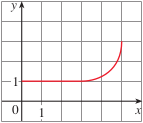
\includegraphics{img/img-0.png}    
        \end{center}    
    Based on the graph, $f$ is both continuous on the interval $[0,5]$ and differentiable on the interval $(0,5)$.
        \[f'(c) = \frac{f(5) - f(0)}{5-0}\]
        \[f'(c) = \frac{3 - 1}{5}\]
        \[f'(c) = \frac{2}{5}\]
    Based on the graph:
        \[c \approx 4\]
    \setcounter{enumi}{10}
    \item Verify that the function satisfies the three hypotheses of Rolle’s Theorem on the given interval. Then find all numbers $c$ that satisfy the conclusion of Rolle’s Theorem.
        \[f(x) = \sin (x/2) \text{, }[\frac{\pi}{2},\frac{3\pi}{2}]\]
    Because $f(x)$ is a trigonometric function, $f(x)$ is both continuous on the interval $[\frac{\pi}{2},\frac{3\pi}{2}]$ and differentiable on the interval $(\frac{\pi}{2},\frac{3\pi}{2})$.
        \[f(\frac{\pi}{2}) = \sin (\pi/4) = \frac{\sqrt{2}}{2}\]
        \[f(\frac{3\pi}{2}) = \sin (3\pi/4) = \frac{\sqrt{2}}{2}\]
    Hence, $f(\frac{\pi}{2}) = f(\frac{3\pi}{2}) = \frac{\sqrt{2}}{2}$. Therefore, there exists $c$ in $(\frac{\pi}{2},\frac{3\pi}{2})$ such as:
        \[f'(c) = 0\]
        \[\frac{1}{2} \cos(c/2) = 0\]
        \[\cos(c/2) = 0\]
        \[c/2 = \pi/2 + k\pi \text{ with k is a integer.}\]
\end{enumerate}

\end{document}